\documentclass[singleside,openright]{uva-bachelor-thesis}

%\usepackage[dutch]{babel}  % uncomment if you write in dutch
\usepackage{graphicx}
\usepackage{url}
\usepackage{enumitem}
\usepackage{multicol}
\usepackage{csquotes}
\usepackage[
style=ieee,
backend=biber
]{biblatex}
\addbibresource{cite.bib}

% Title Page
\title{Bachelor Thesis\\System Architecture}
\author{Matthijs Bos}
\supervisors{Toto van Inge (UvA), Taco Walstra (UvA)}
\signedby{n.a.}


\begin{document}
\maketitle

\tableofcontents

\chapter{Abstract System Architecture}

\section{System overview}


\section{Hardware overview}
From a hardware perspective, the system consists of two main components: a FPGA and a PC which are capable of communicating between each other.

\section{}

\section{Platform components}

PC
\begin{itemize}
\item Package format
\item Desktop client
\begin{itemize}
\item Debugger
\end{itemize}
\end{itemize}

Communication protocol

FPGA
\begin{itemize}
\item FPGA specific driver
\item Communicating component
\item Debugging
\end{itemize}

Workflow



\begin{figure}
\centering
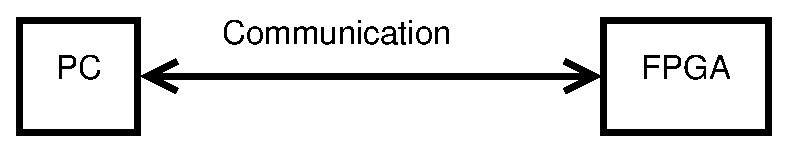
\includegraphics[width=\textwidth]{hardware.eps}
\caption{}
\label{fig:hardware}
\end{figure}

\printbibliography

\end{document}